\documentclass[12pt, a4paper,twoside]{article}

\begin{document}
\label{sec:workDone8thSem}
After the start of this phase, my main aim was towards our big step Data Hashing, hence my whole work during the first month was some literature review and implementing one the papers published recently \cite{DeepHashing}.
The main contributions of the proposed method are shown as follows:
\begin{itemize}
	\item  A novel asymmetric deep structure are proposed. Two streams of deep neural networks are trained to asymmetrically
	learn two different hash functions. The similarity between each pair images are utilized through a pairwise loss according to
	their semantic/label information.
	\item The similarity between the learned features and binary codes are also revealed through an additional asymmetric loss.
	Real-value features and binary codes are bridged through an inner product, which alleviates the binary limitation, better
	preserves the similarity, and speeds up convergence at the training phase
	\item  By taking advantage of these two asymmetric properties, an alternative algorithm is designed to efficiently optimize the
	real values and discrete values.
\end{itemize}
\subsection{Notations and Problem Definition}
In this paper, since there are two streams in the proposed method, they have use the uppercase letters
X = \{$x_{1} , · · · , x_{i} , . . . , x_{N} \}  \epsilon  R^{NXd_{1}Xd_{2}X3}$ and Y = $\{y_{1} , · · · , y_{i}, . . . , y_{N} \} \epsilon R^{NXd_{1}Xd_{2}X3}$  to denote the input images in the first and second deep neural networks, respectively, where N is the number of training samples,
$d_{1}$ and $d_{2}$ are the length and width for each image. Note that, although X and Y are represented with different
symbols, both of them denote the same training data. In our experiments, we only alternatively use training samples X
and Y in the first and second networks. Since our method is supervised learning, the label information can be used.
Let the uppercase letter S $\epsilon \{−1, +1\}$ denote the similarity between X and Y and $S_{i,j}$ is the element in the i-th row and
j-th column in S. Let $S_{i,j} = 1$ if $x_{i}$ and $y_{j}$ share the same semantic information or label, otherwise $S_{i,j} = −1$.

Denote the binary codes as $B = [b_{1} , · · · , b_{i}, . . . , b_{N} ]^T$	 $\epsilon R^{NXk} $
 and the k-bit binary code of the i-th sample as $b_{i} \epsilon \{−1, +1\}^{kX1}$ . The purpose of our model is to learn
two mapping functions $F$ and $G$ to project X and Y into the Hamming space B. $b_{i} = sign(F(x_{i} ))$ and $b_{j} = sign(G(y_{j} ))$,
where sign(·) is an element-wise sign function, and sign(x) =
1 if x ≥ 0, otherwise sign(x) = -1.

Due to the power of deep neural network in data representation, we apply the convolution neural work to learn the hash functions. Specifically, the CNN-F structure is adopted to perform feature learning. In CNN-F model, there are eight layers including five convolutional layers as well as three fully-connected layers. The network structure is listed in Table~\ref{tab:table1111}, where ”f.” means the filter, ”st.” means the convolution stride, ”LRN” means the Local Response Normalization. In order to get the final binary code, we replace the last layer in CNN-F with a k-D vector and the k-bit binary codes are obtained through a sign operation on the output of the last layer. In this paper, CNN-F model is applied to both streams in our proposed asymmetric structure.


\begin{table}[]
\centering
\caption{The Network Structure of CNN-F}
\label{table1111}
\begin{tabular}{|l|c|}
\hline
Layer & Structure                                       \\ \hline
conv1 & f. 64 × 11 × 11; st. 4×4; pad. 0; LRN.; ×2 pool \\ \hline
conv2 & f.265 × 5 × 5; st. 1×1; pad. 2; LRN.; ×2 pool   \\ \hline
conv3 & f. 265 × 3 × 3; st. 1×1; pad. 1                 \\ \hline
conv4 & f.265 × 3 × 3; st. 1×1; pad. 1                  \\ \hline
conv5 & f. 265 × 3 × 3; st. 1×1; pad. 1; ×2 pool        \\ \hline
full6 & 4096                                            \\ \hline
full7 & 4096                                            \\ \hline
full8 & k-bit hash code                                 \\ \hline
\end{tabular}
\end{table}

\begin{figure}[htbp]
\centering
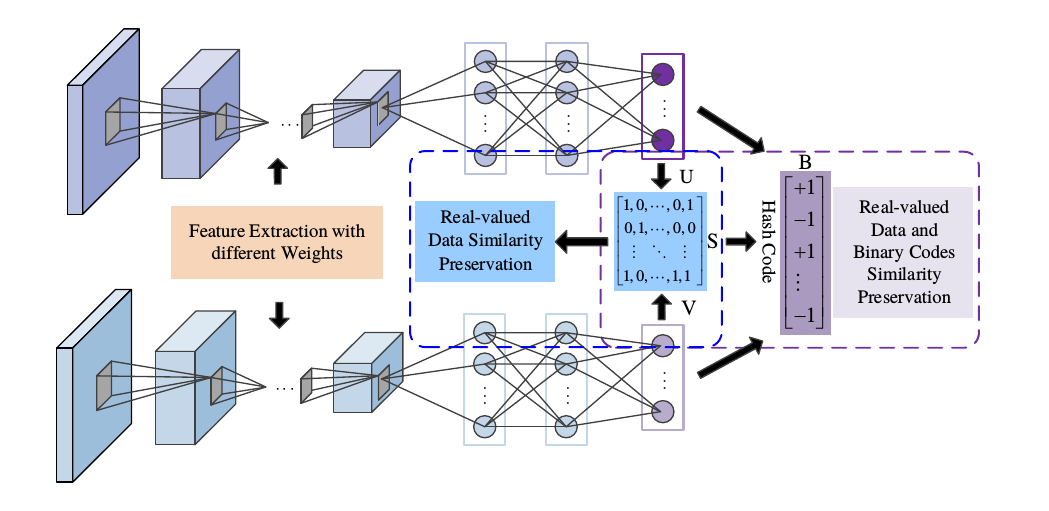
\includegraphics[scale=0.6]{images/cnnNetwork}
\caption{ The framework of the proposed method. Two streams with five convolution layers and two full-connected layers are used for feature extraction.
}\label{fig:figure111}
\end{figure} 



\subsection{Dual Asymmetric Deep Hashing Learning}
	The main framework of the proposed method is shown in Fig~\ref{fig:figure111}. As we can see, there are two end-to-end neural networks to discriminatively represent the inputs. For a pair of outputs F and G in these two streams, their semantic
information is exploit through a pairwise loss according to their predefined similarity matrix. Since the purpose is to
obtain hash functions through the deep networks, the binary code B is also generated by minimizing its distance between
F and G. Furthermore, in order to preserve the similarity between the learned binary codes and real-value features, and
alleviate the binary limitation, another asymmetric pairwise loss is introduced by using the inner product of the hash codes
B and learned features $F (G)$

Denote $f (x_{i}, W_{f} )$ $\epsilon R^{kX1}$ as the output of the i-th sample in the last layer of the first stream, where $W_{f}$ is the parameter of the network. To simplify the notation, we use $f_{i}$ to replace $f (x_{i}, W_{f} )$. Similarly, we can obtain the output $g_{j}$corresponding to the j-th sample under the parameter $W_{g}$ in the second network. Thus, the features $F = [f_{1} , · · · , f_{i} , f_{n} ]^T \epsilon R^{nXk}$ and $G = [g_{1}, · · · , g_{i} , g_{n}]^T \epsilon R^{nXk}$ corresponding to the first and second networks are then gained.
To learn an accurate binary code, we set $sign(f_{i})$ and $sign(g_{i})$ to be close to their corresponding hash code $b_{i}$ . A
general way is to minimize the L2 loss between them.

\begin{equation}
	    min \vert \vert sign(f_{i}) - b_{i} \vert \vert ^2 _{2} + \vert \vert sign(g_{i}) - b_{i} \vert \vert^2_{2}
\label{eq9}
\end{equation}
However, it is difficult to make a back-propagation for the gradient with respect to $f_{i}$ or $g_{i}$ since their gradients are zero anywhere. In this paper, we apply tanh(·) to softly approximate the sign(·) function. Thus, equation is transformed into

\begin{equation}
	    min \vert \vert tanh(f_{i}) - b_{i} \vert \vert ^2 _{2} + \vert \vert tanh(g_{i}) - b_{i} \vert \vert^2_{2}
\label{eq10}
\end{equation}

Although previous equation achieves to approximate discrete codes but the similarity between the binary codes and real-value features is ignored. To tackle this problem, another asymmetric pairwise loss is introduced.

\begin{equation}
	    min \vert \vert tanh({f_{i}}^T)b_{j} - kS_{ij} \vert \vert ^2 _{2} + \vert \vert tanh({g_{i}}^T)b_{j} - kS_{ij} \vert \vert^2_{2}
\label{eq11}
\end{equation}

In above Eq., the similarity between the real-valued data and binary codes is measured by their inner product. It is easy to observe that above Eq. not only encourages the $tanh(f_{i} ) (tanh(g_{i} ))$ and $b_{i}$ to be consistent, but also preserve the similarity between them.
Jointly taking all the equations into account, the objective function can be obtained as follows:


\begin{equation}
	\begin{aligned}
	    min_{F,G,B}  L = \vert \vert tanh(F)B^T - kS \vert \vert ^2 _{F} + \vert \vert tanh(G)B^T - kS \vert \vert^2_{F} 
	    \\- \tau \sum\limits_{i,j=1}^n (S_{ij}\theta_{ij} - log(1 + \exp^{\theta_{ij}})) 
	    \\+ \gamma (\vert \vert tanh(F) - B \vert \vert^2_{F} + \vert \vert tanh(G) - B\vert \vert^2_{F}) 
	    \\+ \eta(\vert \vert tanh(F)^T1\vert\vert^2_{F} + \vert\vert tanh(G)^T1 \vert \vert^2_{F})
	   \end{aligned}
\label{eq12}
\end{equation}


where $\tau$ , $\gamma$ and $\eta$ are the non-negative parameters to make a trade-off among various terms. Note that the purpose of the
forth term $\vert \vert tanh(F)^T1 \vert \vert^2_{F} + \vert \vert tanh(G)^T1 \vert \vert^2_{F}$ in the objective. function is to maximize the information provided by each bit. In detail, this term makes a balance for each bit, which encourages the number of -1 and +1 to be approximately similar among all training samples.


\end{document}
 
 
 
